\section{Model I: Analysis Model of Submersible Loss of Contact Process}

\begin{figure}[htbp]
  \centering
  \begin{subfigure}[b]{0.48\textwidth}
    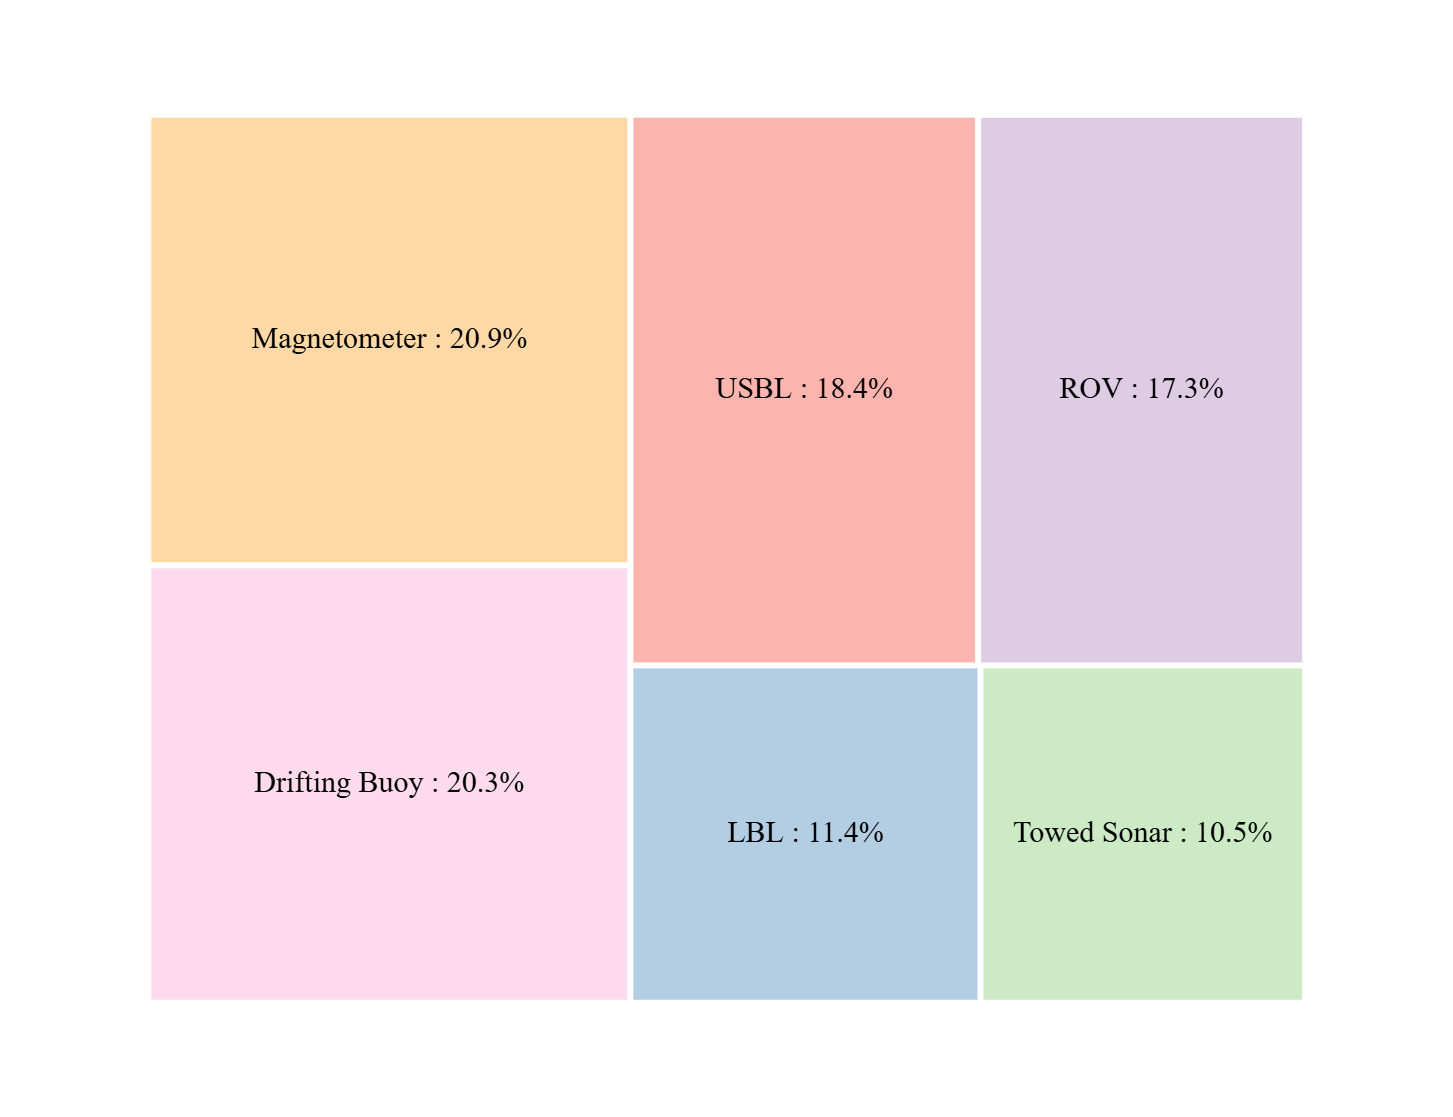
\includegraphics[width=\textwidth]{../figures/treemap1.png}
    \caption{tree map 1}
    \label{fig:treemap1}
  \end{subfigure}
  \hfill
  \begin{subfigure}[b]{0.45\textwidth}
    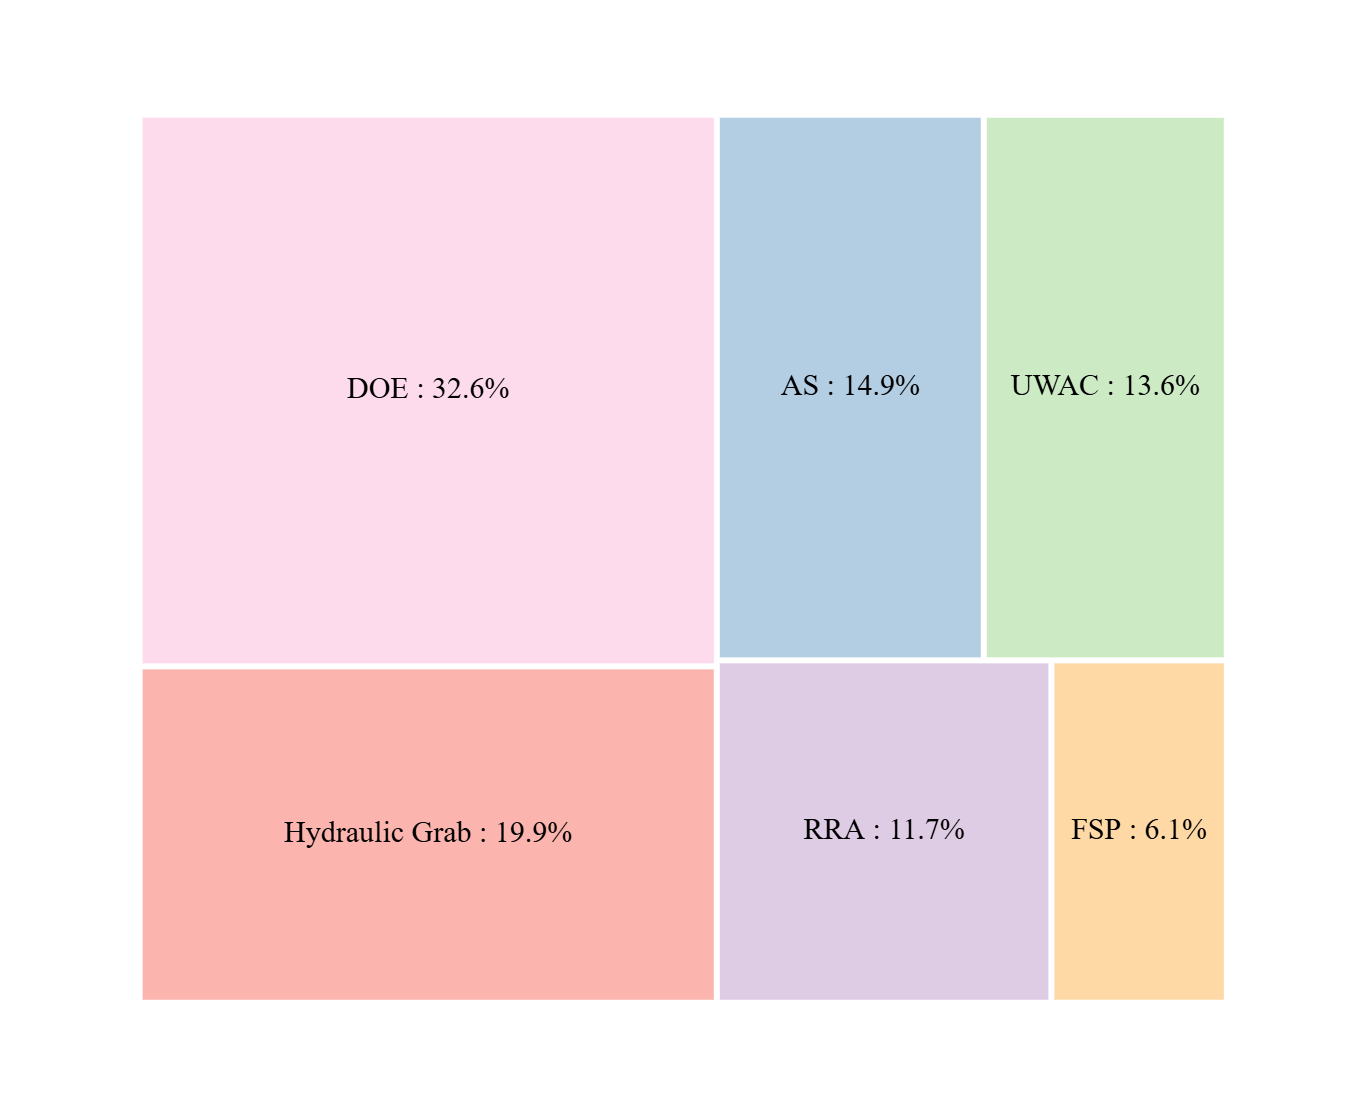
\includegraphics[width=\textwidth]{../figures/treemap2.png}
    \caption{tree map 2}
    \label{fig:treemap2}
  \end{subfigure}
  \caption{two examples of tree map}
  \label{fig:two_treemaps}
\end{figure}


\begin{figure}[htbp]
  \centering
  \begin{subfigure}[b]{0.45\textwidth}
    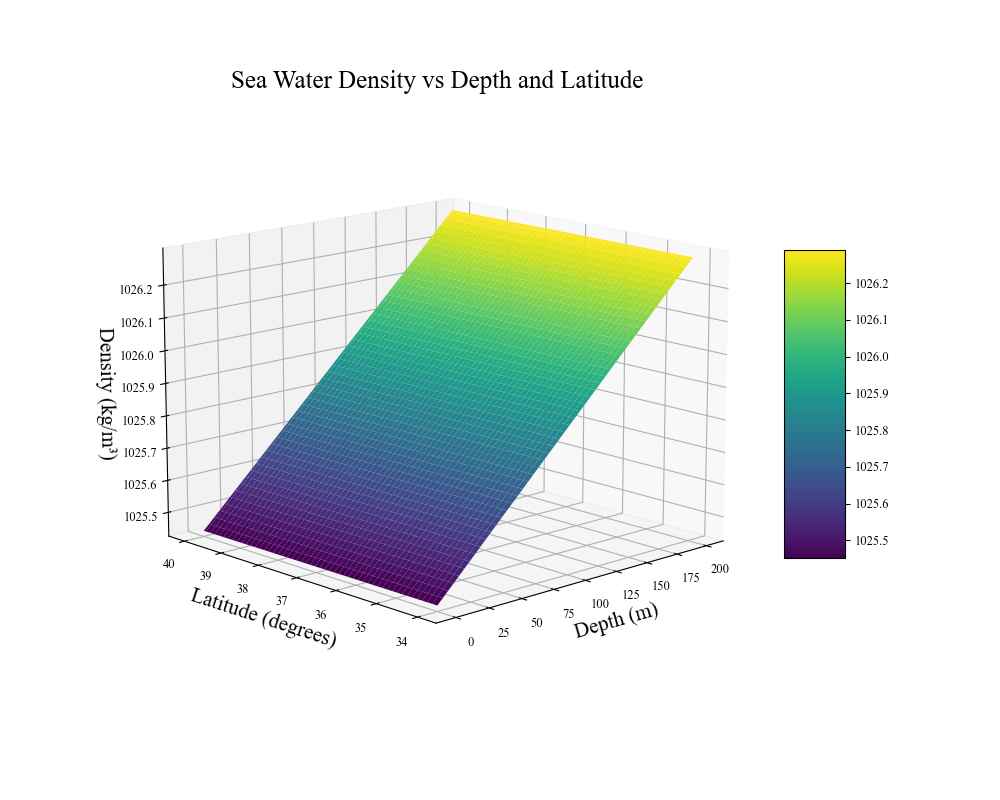
\includegraphics[width=\textwidth]{../figures/Density1.png}
    \caption{density 1}
    \label{fig:density1}
  \end{subfigure}
  \hfill
  \begin{subfigure}[b]{0.45\textwidth}
    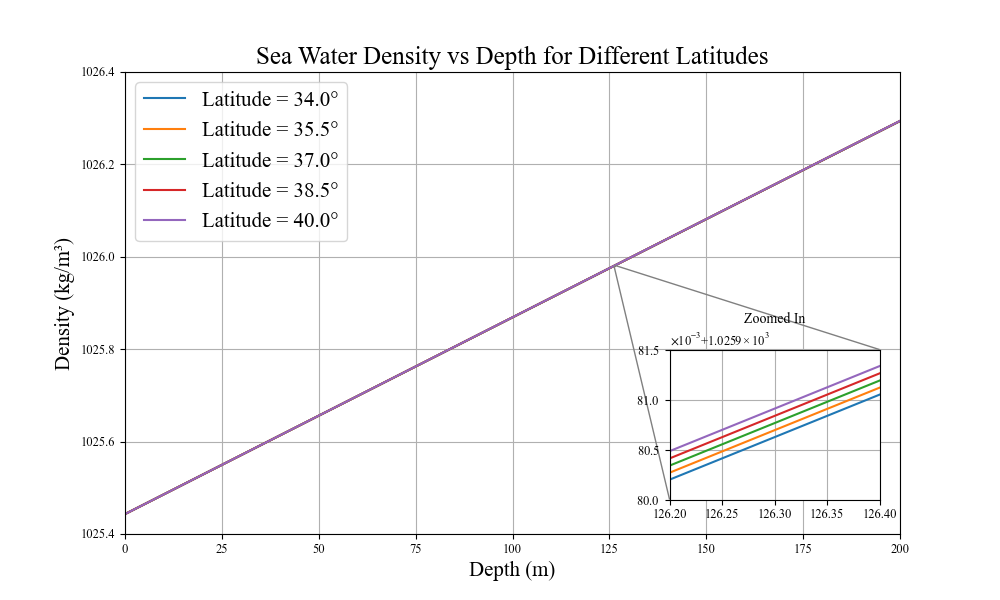
\includegraphics[width=\textwidth]{../figures/Density2.png}
    \caption{density 2}
    \label{fig:density2}
  \end{subfigure}
  \caption{density of sea}
  \label{fig:density of sea}
\end{figure}

